\chapter{Analíticas de Elasticsearch y Dash}
\label{analiticas}
En este capítulo se explica la recogida de las diferentes sondas en Unibotics con la base de datos Elasticsearch, la visualización de la información con el \textit{framework} web Dash y la validación experimental de este proceso.
\section{Recogida de sondas}
La primera parte de este proceso ha consistido en la recogida de diferentes sondas para lo cual se ha decidido utilizar la herramienta de Elasticsearch por las ventajas que ofrece explicadas en el capitulo 3. Para comenzar hay que instalar Elasticserach en local, se puede descargar directamente desde la página web de elastic\footnote{https://www.elastic.co/es/elasticsearch/} o a través del administrador de paquetes pip con el comando \texttt{pip install elasticsearch}.\\

En este proyecto se ha utilizado docker, un contenedor a nivel de sistema operativo para Elasticsearch, primero hay que descargar la imagen de Elasticsearch con la versión deseada en este caso se ha utilizado la 7.12.0, el comando para descargar la imagen es:
{\footnotesize
		\begin{verbatim}
			docker pull docker.elastic.co/elasticsearch/elasticsearch:7.12.0
		\end{verbatim}
		}
Para ejecutar el contenedor con la imagen descargada se utiliza el siguiente comando:
{\footnotesize
		\begin{verbatim}
			docker run --name=AcademyElastic -p 9200:9200 -p 9300:9300
            -e "discovery.type=single-node" 
            docker.elastic.co/elasticsearch/elasticsearch:7.12.0
		\end{verbatim}
		}
        
  Una vez ya puesto en marcha el contenedor de Elasticsearch ya tenemos nuestra base de datos donde se guardaran las sondas, para hacer solicitudes se podrá hacer mediante \textit{REST APIs}, un ejemplo sería introducir en el navegador la siguiente URL: \texttt{http://localhost:9200/}.\\
  
  El siguiente paso es la integración de Elasticseach en el proyecto de Django, para ellos se hará uso de la librería \texttt{django-elasticsearch-dsl}, además se ha modificado el archivo de configuración del proyecto, \texttt{settings.py},  añadiendo la librería a las aplicaciones instaladas y creando una nueva variable llamada \texttt{ELASTICSEARCH\_DSL} donde se indica el servidor de Elasticsearch con el que se tiene que conectar y sincronizar.\\
  
  Una vez ya conectados, el servidor de Django y Elasticsearch, se ha definido y configurado los índices donde se guardaran las sondas, para ellos se ha creado un nuevo archivo llamado \texttt{probe.py}. Al definir un índice, se determinan los nombres de cada dato del índice con su tipo, también se puede configurar el índice, por ejemplo poniendo el número de\textit{ shards }o el número de réplicas. Un ejemplo de la definición de un índice sería este: \\

\begin{lstlisting}
   from django_elasticsearch_dsl import Document, Date, Text, Double
   
   class SessionDocument(Document):
    		username = Text()
  	  		start_date = Date()
   			end_date = Date()
    		duration = Double()
    		client_ip = Text()
    		browser = Text()
    		country = Text()
    		alpha_2 = Text()
    		alpha_3 = Text()
    		continent = Text()
    		class Index:
        		name = 'session_log'
        		settings = {
            			'number_of_shards': 1,
           				'number_of_replicas': 0
        }
\end{lstlisting} 
 \newpage
Para este proyecto se han definido cuatro índices diferentes:

\begin{itemize}
\item \texttt{session\_log}: índice que recoge las sondas relativos a las sesiones. Consta de los campos de inicio y fin de sesión, duración de la sesión, la IP, el \textit{browser} (aporta información sobre el sistema operativo, navegador y dispositivo utilizado), el continente y país del usuario, así como el nombre del usuario.
\item \texttt{exercises\_log}: índice que recoge las sondas relativos a los diferentes ejercicios. Esta compuesto por la fecha de entrada en un ejercicio, la fecha de salida del ejercicio, la duración total, el nombre del ejercicio y el usuario.
\item \texttt{style\_log}: índice que recoge los datos sobre la evaluación del estilo del código de los ejercicios. Este índice esta formado por el campo de la fecha en la que se realiza la evaluación, el nombre del ejercicio, la puntuación sobre 100 y el nombre del usuario.
\item \texttt{efficacy\_log}: índice que recoge los datos sobre la evaluación de la eficacia del código de los ejercicios. Los campos son iguales que en el índice de \texttt{style\_log}.
\end{itemize}

Ya definidos los diferentes índices se importan al archivo \texttt{views.py} para poder crearlos.Las sondas de sesión se han guardado para usuarios registrados por lo cual en el momento que hacen \textit{login} se crea el índice de esta manera:
\\
{\footnotesize
\begin{verbatim}
    probe_session = SessionDocument(username=username,start_date=datetime.now(),
                                    end_date=datetime.now(),duration=0, client_ip=ip,
                                    browser=request.META['HTTP_USER_AGENT'],
                                    country=location_info["country_name"],
                                    alpha_2=location_info["alpha_2"], 
                                    alpha_3=location_info["alpha_3"],
                                    continent=location_info["continent"])
    probe_session.save()
\end{verbatim}
}
\newpage
Gracias al objeto HTTP Request que recibe el fichero \texttt{views.py} obtenemos la información del nombre del usuario, la IP y el \textit{user-agent} el cual nos dirá el sistema operativo, el navegador o el dispositivo que utiliza el usuario. Para la localización se ha creado una función que a partir de la IP muestra la ubicación. En un principio los campos de fin de sesión y duración se inicializan con la fecha actual y 0 respectivamente, una vez que el usuario haga \textit{logout} o finalice su sesión por inactividad estos campos se modificarán como se muestra a continuación:\\
{\footnotesize
\begin{verbatim}
    s = Search(index="session_log").query('match', username=request.user.username) \
                                    .sort({"start_date": {'order':'desc'}})[0]
    for hit in s:
        end = datetime.now()
        Elasticsearch(settings.ELASTICSEARCH_DSL['default']['hosts']) \
                        .update(index="session_log", id=hit.meta.id,
                                body={"doc": {'end_date': end,
                                'duration':(end - datetime \
                                    .strptime(hit.start_date,'%Y%m%dT%H:%M:%S.%f')) \
                                    .total_seconds()}})
\end{verbatim}
}
\\
Las sondas relativas a los ejercicios se guardan una vez accedido al ejercicio y como pasaba con las sesiones, cuando el usuario salga del ejercicio se modificarán los datos de duración y fin del ejercicio. En este punto se ha tenido en cuenta si el usuario recarga la página cuando esta en un ejercicio ya que al volver a cargar el ejercicio se crea una sonda nueva que no es necesaria por lo cual se elimina de la siguiente manera:\\
\\
{\footnotesize
\begin{verbatim}
   es = Search(index="exercises_log").query('match', duration=0)  \
   				            .query('match', username=request.user.username)  \
        					                .sort({"start_date": {'order':'desc'}})
    for hit in es:
        Elasticsearch(settings.ELASTICSEARCH_DSL['default']['hosts'])  \ 
    				                        .delete(index="exercises_log", id=hit.meta.id)
\end{verbatim}
}
\\
Para las sondas de la evaluación del estilo del código ya había incorporado en la plataforma un botón que evalúa el estilo donde se recoge la puntuación para Elasticsearch, pero en el caso de la sonda de evaluación de la eficacia del código se ha tenido que crear un nuevo botón el cual ejecuta el código como si fuera el botón de \textit{play} y al cabo de un tiempo determinado para cada ejercicio recoge la nota obtenida. En el caso de que el usuario vuelva a pulsar el botón no se guardará la sonda.


En este proceso de recogida de sondas y su grabación ha sido muy útil la utilización de la API que proporciona Elasticsearch para poder depurar y comprobar los datos que se estaban almacenando. Utilizando por ejemplo la URL \texttt{http://127.0.0.1:9200/session\_log/\_search/?size=10000&pretty} se comprueba las sondas de sessiones.\\

Por último se creó una base de datos de prueba de Elasticsearch para poder comenzar a trabajar antes de tener los datos reales los cuales llevan tiempo recoger. La base de datos Elasticsearch dummy se ha creado gracias a las librerías de python Faker\footnote{https://faker.readthedocs.io/en/master/} y Tornado\footnote{https://www.tornadoweb.org/en/stable/} en ella se puede modificar las sondas como por ejemplo el número de sondas, de réplicas o de \textit{shards}. Esto ayudará a futuros desarrolladores a utilizar la base de datos de Elasticsearch. En la figura\ref{fig:dummy} se muestra como ejemplo el resultado de la sonda de evaluación de estilo de la base de datos de prueba.


\begin{figure}[H]
    \centering
    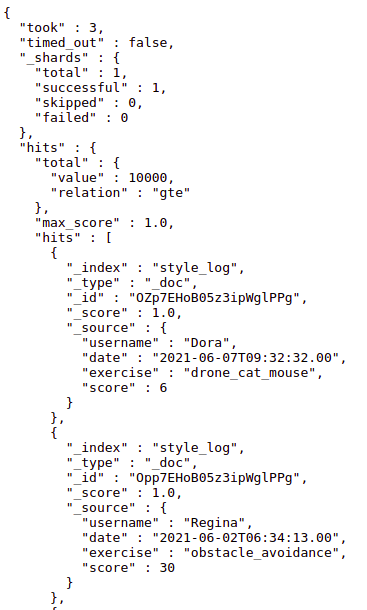
\includegraphics[width=6cm, keepaspectratio]{img/dummy.png}
    \caption{Elasticsearch dummy}
    \label{fig:dummy}
\end{figure}

\section{Visualización de la información}

Dash es un \textit{framework} web que ayuda a la creación de aplicaciones para poder hacer análisis como se explica en el capítulo 3. En este Trabajo de fin de grado se ha decidió utilizar esta herramienta para la visualización de las sondas recogidas en Elasticsearch.Estas visualizaciones se unen con la plataforma de Unibotics a través de un enlace en el menú de esta.\\

Una vez accedemos a la aplicación se encuentra una barrera de seguridad donde solo podrán entrar los usuarios registrados en la plataforma por lo cual habrá que iniciar sesión. Una vez iniciada la sesión gracias a la base de datos MySQL que ya tenía la plataforma, se sabe si el usuario es un administrador o no. Esto hace que según si eres administrador o no se muestre un menú u otro, en el caso de los administradores podrán ver la información de todas las sondas y en el caso de que no lo seas solo se podrá ver las puntuaciones que ha recibido dicho usuario en los diferentes ejercicios, tanto de estilo como de eficacia. En la figura \ref{fig:menu} se puede ver el menú que un administrador vería.

\begin{figure}[H]
    \centering
    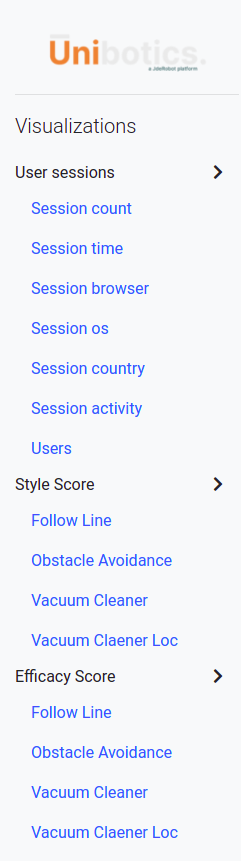
\includegraphics[width=3cm, keepaspectratio]{img/menu.png}
    \caption{Menú de un administrador en Dash}
    \label{fig:menu}
\end{figure}


Gracias a las bibliotecas de Dash mencionadas en el capítulo 3 se ha dado estilo y formato a la aplicación, también se ha hecho uso de la \textit{cookies }del navegador para comprobar si se esta autorizado y si es un administrador de la plataforma.\\

Como Dash trabaja con \textit{Dataframes} el primer paso al crear las diferentes gráficas ha sido la conversión de los datos almacenados en Elasticsearch a dataframes gracias a la biblioteca de Pandas. Un ejemplo de la realización de esta conversión es:

{\footnotesize
\begin{verbatim}
  s = Search(using=es, index="session_log")
  results = [hit.to_dict() for hit in s.scan()]
  df  = pd.DataFrame(results)
\end{verbatim}
}
\\

Con la biblioteca \texttt{dash\_core\_components} se ha creado los filtros que algunas de las gráficas poseen. El primer filtro es por fechas, con los callbacks que Dash proporciona se modificará las gráficas según las fechas introducidas, puede ser un filtrado entre dos fechas o una única fecha de comienzo o de final. El código de filtrado ha sido:

{\footnotesize
\begin{verbatim}
 if start_date is not None and end_date is not None:
        df=df.loc[(df['start_date'] > start_date) & (df['start_date'] <= end_date)]
elif start_date is not None:
        df=df.loc[(df['start_date'] > start_date)]
elif end_date is not None:
        df=df.loc[(df['start_date'] <= end_date)]
\end{verbatim}
}
\\

Otro filtro también presente en algunas gráficas como en la actividad es el filtro de los usuarios. Este filtro se encuentra además en las gráficas de las evaluaciones de estilo y eficacia del código pero solo para los administradores, así podrán ver las puntuaciones de los diferentes usuarios. Para este filtro se hace uso de las sondas de sesiones (convertidas en dataframes) recogiendo los nombres de los usuarios de forma única y en el caso que también se quiera ver todos los valores de los usuarios en conjunto se ha añadido una opción de 'Total'. El código es el siguiente:
\newpage
{\footnotesize
\begin{verbatim}
	s = Search(using=es, index="session_log")
    results = [hit.to_dict() for hit in s.scan()]
    df  = pd.DataFrame(results)
    df = df[df['username'].notna()]
    users = df['username'].unique()
    if not exercises:
        users = np.insert(users,0,'Total')
    return users
\end{verbatim}
}
\\
\begin{figure}[H]
    \centering
    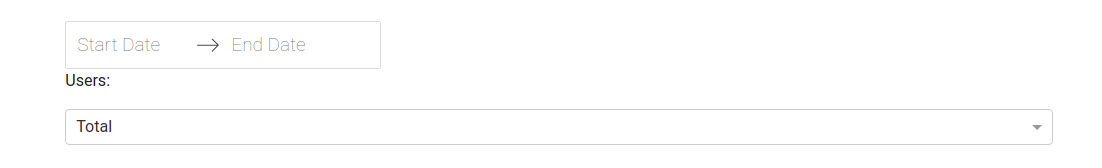
\includegraphics[width=16cm, keepaspectratio]{img/filtros.png}
    \caption{Filtros utilizados en Dash}
    \label{fig:filtros}
\end{figure}

Cuando ya se tienen los datos que se quieren visualizar en formato Dataframe, Dash hace uso de plotly para la creación de las gráficas. Plotly ofrece una gran variedad de gráficas que se pueden utilizar en Dash. Adicionalmente se puede combinar varias gráficas en los mismos ejes, haciendo más sencillo la correlación entre datos. El código, por ejemplo, para crear la gráfica de número de sesiones por día es:\\
{\footnotesize
\begin{verbatim}
fig = px.line(df, x='start_date', y='count')
    fig.update_layout(xaxis_tick0=df['start_date'][0], xaxis_dtick=86400000 * 2)
    fig.add_trace(go.Scatter(x=df["start_date"].tolist(), y=df["count"].tolist(),
                             mode="markers", textposition="top center", 
                             name="Number of sessions",
                             text=df["count"].tolist()))
return fig
\end{verbatim}
}
\\
\newpage

\section{Validación experimental}

En esta sección se muestra los resultados finales de las analíticas con datos reales de la plataforma de Unibotics, donde se verán las diferentes gráficas creadas tanto para administradores como para los usuarios, así como una explicación de lo que representan.\\

La primera gráfica creada se muestra en la figura \ref{fig:sesion} , donde se esta representando en el eje x el tiempo y en el eje y el número de sesiones, dando como resultado una gráfica de linea a la cual se le ha añadido puntos para una mejor visualización. En resumen se pueden ver el numero de sesiones por día independientemente del usuario. La gráfica nos va a dar información de cuando la plataforma esta más visitada, por ejemplo,  en este caso se puede ver como en verano ha habido una bajada de inicios de sesión.



\begin{figure}[H]
    \centering
    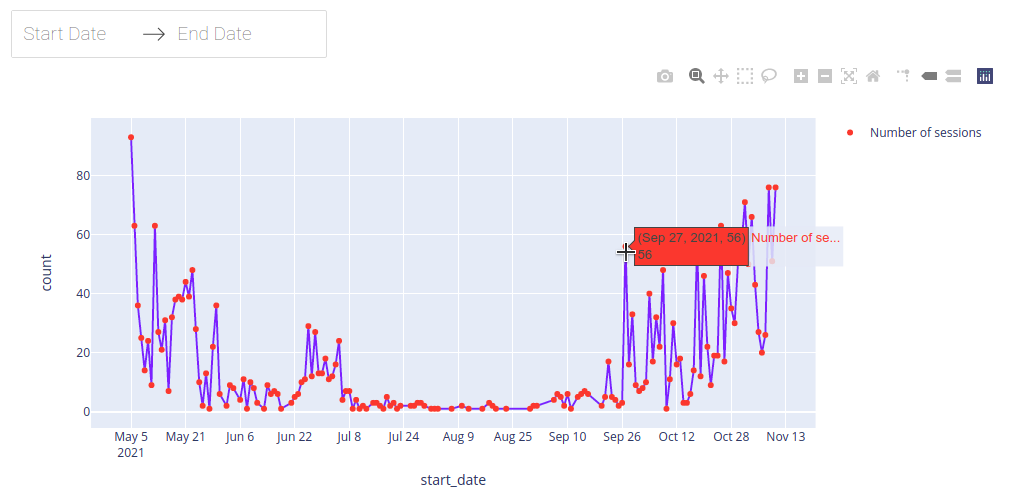
\includegraphics[width=19cm, keepaspectratio]{img/sesion.png}
    \caption{Gráfico sesiones por día}
    \label{fig:sesion}
\end{figure}
\newpage
La figura \ref{fig:time} muestra una gráfica de barras donde en el eje x esta el tiempo y en el eje y la duración total en minutos que los usuarios han estado en la plataforma. Se puede ver que en los mismos ejes hay otra gráfica de linea que señala la media por día. Aquí podemos comprobar que a veces la media coincide con la duración total debido a que solo ha tenido que haber una sesión en ese día.



\begin{figure}[H]
    \centering
    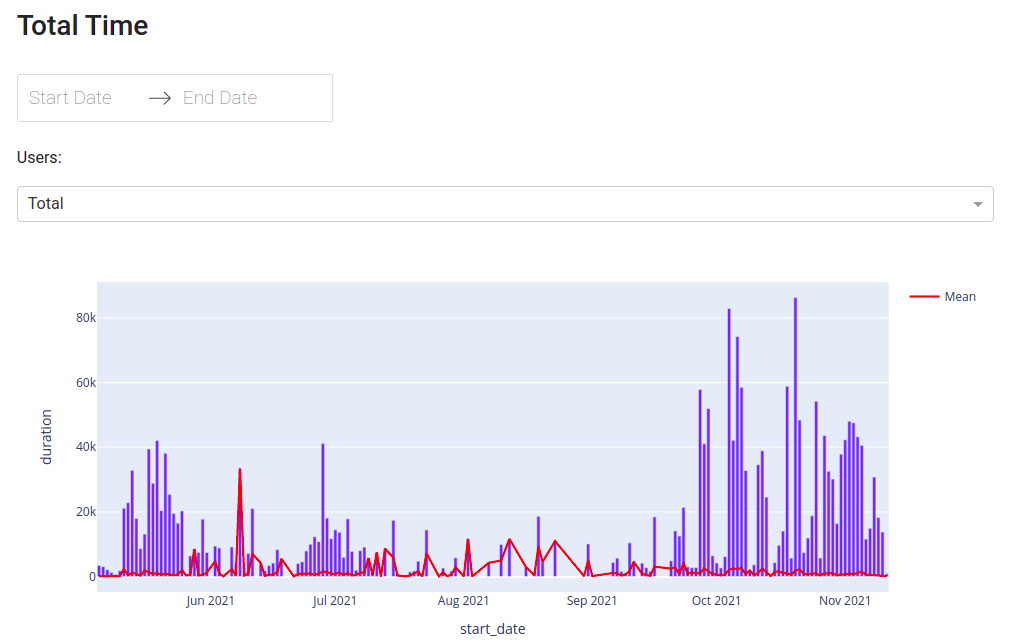
\includegraphics[width=18cm, keepaspectratio]{img/time.png}
    \caption{Gráfico de tiempo en Unibotics}
    \label{fig:time}
\end{figure}
Esta gráfica se puede filtrar tanto por fechas como por usuarios, pudiendo ver el tiempo dedicado de un usuario y la media total del tiempo que usa Unibotics como se puede ver en la figura \ref{fig:time_user}.

\begin{figure}[H]
    \centering
    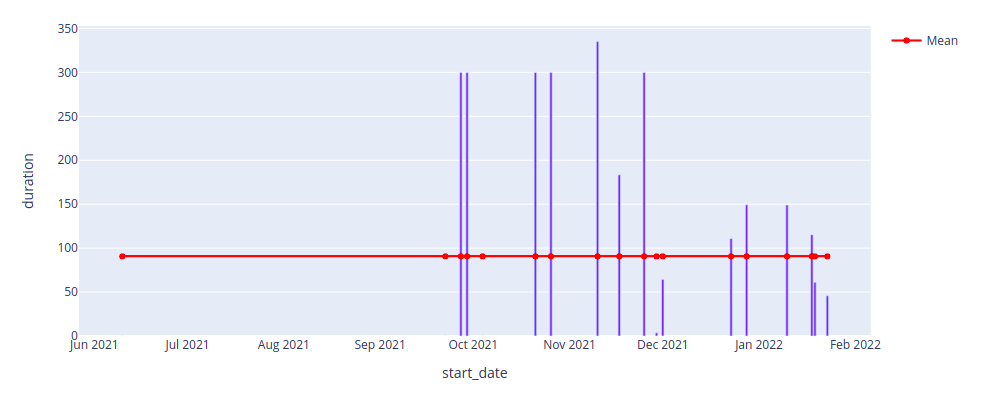
\includegraphics[width=18cm, keepaspectratio]{img/time_user.png}
    \caption{Gráfico de tiempo en Unibotics de un usuario}
    \label{fig:time_user}
\end{figure}

La siguiente gráfica circular mostrada en la figura \ref{fig:browser} muestra desde que navegador los usuarios utilizan Unibotics en formato porcentaje con un filtro de fechas. En este caso se ve que una gran parte de inicio de sesiones es a través del navegador de Chrome.



\begin{figure}[H]
    \centering
    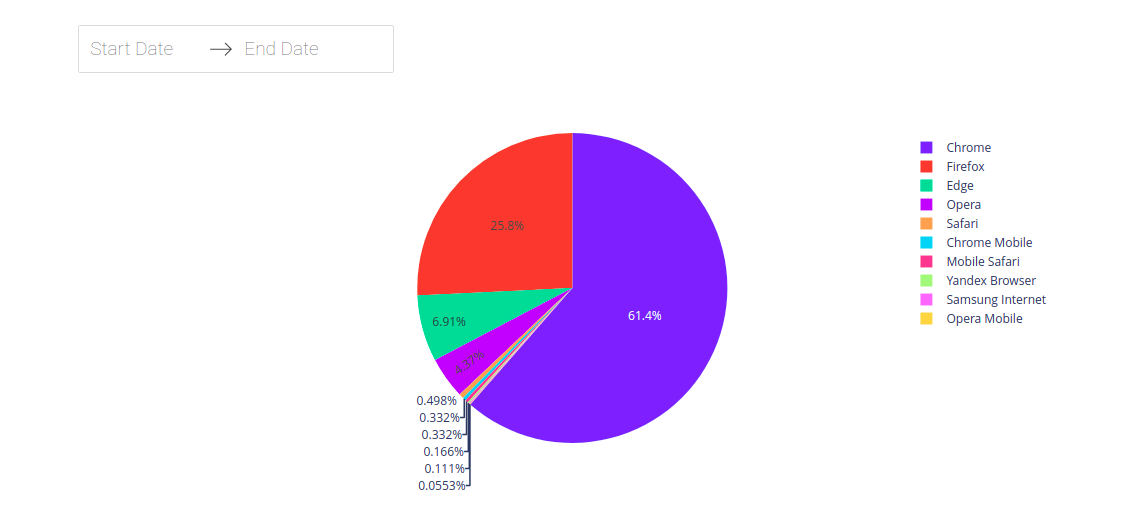
\includegraphics[width=19cm, keepaspectratio]{img/browser.png}
    \caption{Gráfico de navegadores}
    \label{fig:browser}
\end{figure}
\newpage
La gráfica para saber el sistema operativo que utilizan los usuarios es del mismo estilo que la gráfica de los navegadores como se puede ver en la figura \ref{fig:os}. Ambas gráficas tienen filtro por fechas.


\begin{figure}[H]
    \centering
    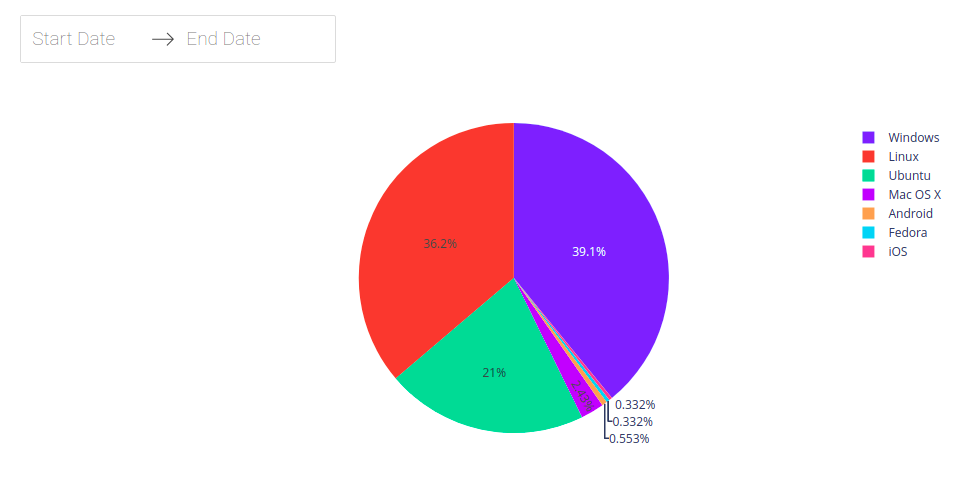
\includegraphics[width=17cm, keepaspectratio]{img/os.png}
    \caption{Gráfico de sistemas operativos}
    \label{fig:os}
\end{figure}
\newpage
En la figura \ref{fig:mundo} se muestra un mapa geográfico donde cada punto es el lugar donde los usuarios inician sesión. El tamaño de los puntos depende de la cantidad de sesiones, cuanto mayor sea el punto más sesiones hay. A la derecha se encuentra una leyenda con los países, se puede seleccionar uno o varios países en la leyenda para que solo se vean ellos en el mapa. Se puede filtrar por fechas.



\begin{figure}[H]
    \centering
    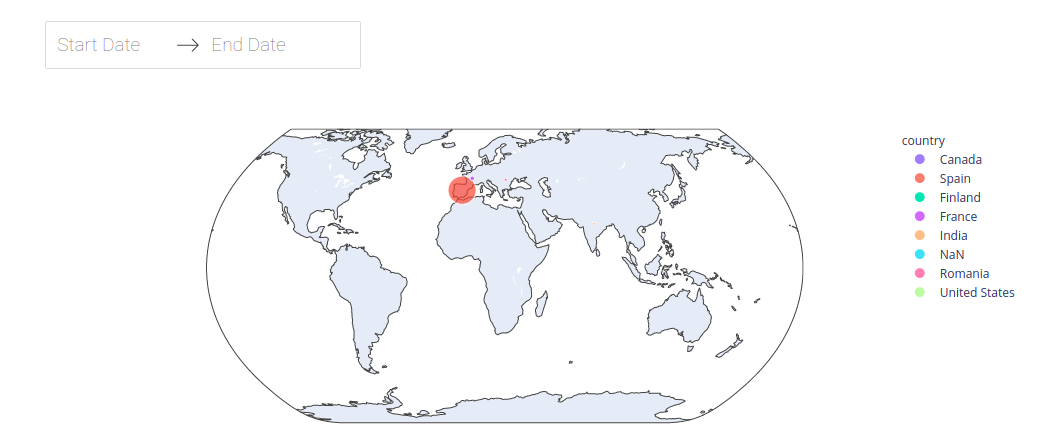
\includegraphics[width=17cm, keepaspectratio]{img/mundo.png}
    \caption{Mapa geográfico de sesiones}
    \label{fig:mundo}
\end{figure}

En la siguiente gráfica que se ve en la figura \ref{fig:activity} representa un mapa de calor con la actividad de los usuarios. Esta dividido en cuadrados que representan cada día de un año, cuanto más intenso es el color verde más sesiones ha habido, ha medida que disminuyen las sesiones la intensidad también baja. Tiene un filtro por usuario para ver la actividad por usuarios únicos.


\begin{figure}[H]
    \centering
    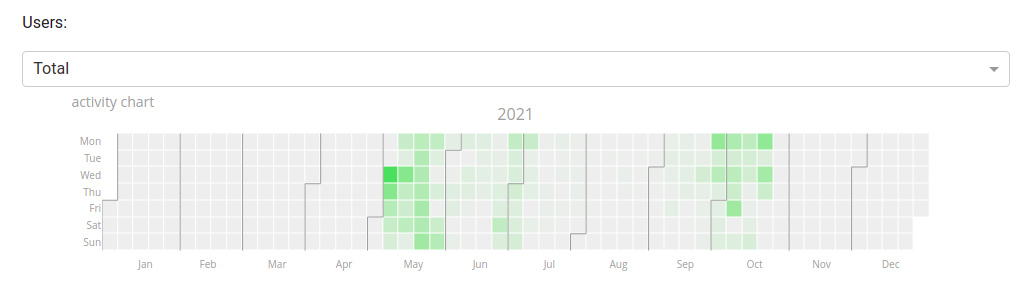
\includegraphics[width=17cm, keepaspectratio]{img/activity.png}
    \caption{Mapa de calor sesiones}
    \label{fig:activity}
\end{figure}
\newpage
La última gráfica única para administradores que se muestra en la figura \ref{fig:activity}, es la de usuarios, donde se representa el número total de usuarios que son activos, el número de usuarios que han sido activos en los últimos 2 meses, una gráfica de linea donde se ven el número de registros por cada día, otra gráfica con los registros acumulados por días y la última gráfica se muestra los usuarios activos en los últimos 2 meses, es decir cada día se comprueba cuantos usuarios han iniciado sesión desde 2 meses atrás hasta ese día concretamente. Cada una de estas gráficas contiene su propio filtrado por fechas.

\begin{figure}[H]
    \centering
    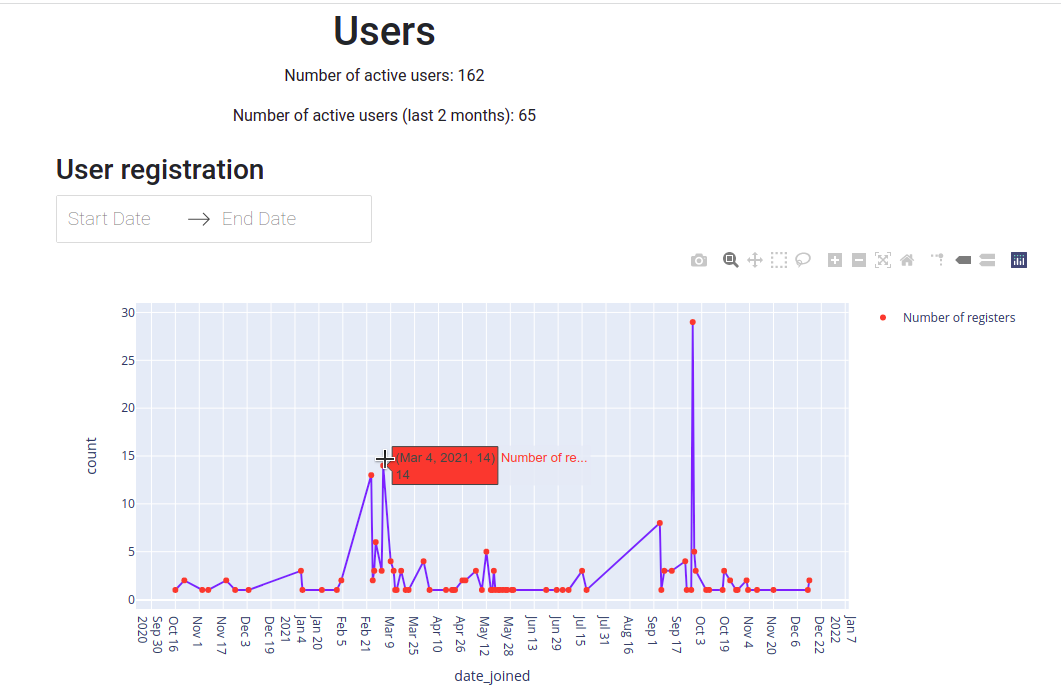
\includegraphics[width=17cm, keepaspectratio]{img/users.png}
    \caption{Gráficas relativas a los usuarios}
    \label{fig:users}
\end{figure}

\newpage
Las siguientes gráficas son las puntuaciones de estilo y eficacia donde los usuarios podrán ver las suyas y los administradores las de cualquier usuario. Actualmente las evaluaciones solo están disponibles en cuatro ejercicios representadas en una gráfica donde cada punto es una nota recibida. La gráfica mostrada en la figura \ref{fig:score} es un ejemplo de las notas de estilo de un usuario de la base de datos de prueba en el ejercicio \textit{follow\_line}. Las gráficas de los demás ejercicios son iguales como las de las puntuaciones de eficacia.



\begin{figure}[H]
    \centering
    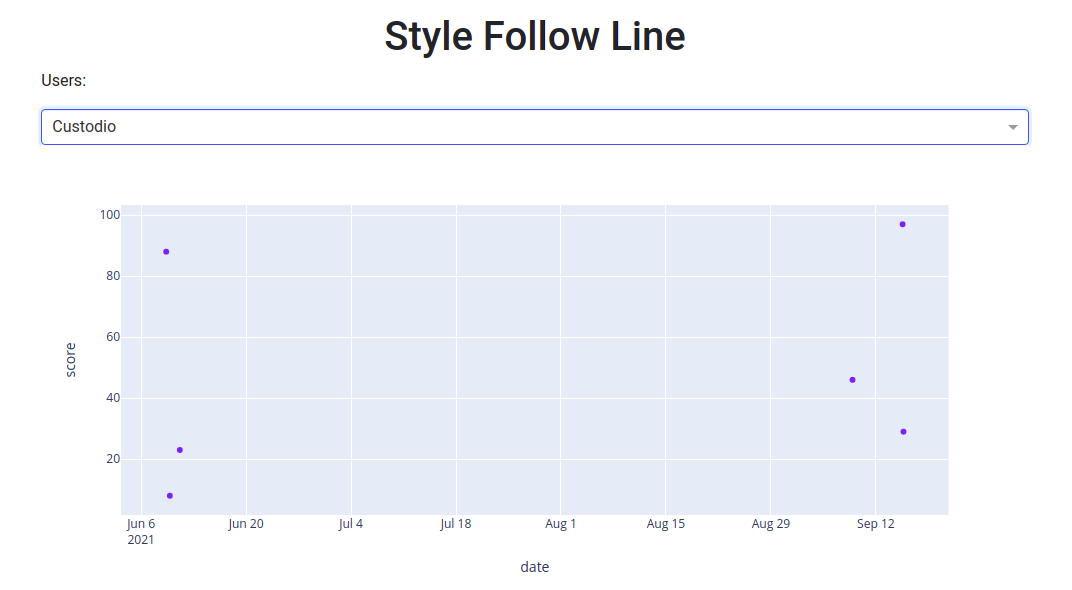
\includegraphics[width=17cm, keepaspectratio]{img/score.png}
    \caption{Gráfica de puntuación de estilo}
    \label{fig:score}
\end{figure}

En todas estas gráficas se pueden ampliar, disminuir o pasar el cursor sobre alguno de sus puntos dándote una mayor información.









